\documentclass[article,10pt]{scrartcl}
\usepackage{graphicx}
\usepackage{amsmath}
\usepackage{tikz}
\usepackage{vmargin}
\setmarginsrb{1.3cm}{1.3cm}{1.3cm}{1.3cm}{1.3cm}{1.3cm}{1.3cm}{1.3cm}
\setlength{\parindent}{0cm}
\usepackage{color}
\usepackage{listings}
\usepackage{hyperref}

% python script syntax taken from 
% http://widerin.org/blog/syntax-highlighting-for-python-scripts-in-latex-documents
\definecolor{Code}{rgb}{0,0,0}
\definecolor{Decorators}{rgb}{0.5,0.5,0.5}
\definecolor{Numbers}{rgb}{0.5,0,0}
\definecolor{MatchingBrackets}{rgb}{0.25,0.5,0.5}
\definecolor{Keywords}{rgb}{0,0,1}
\definecolor{self}{rgb}{0,0,0}
\definecolor{Strings}{rgb}{0,0.63,0}
\definecolor{Comments}{rgb}{0,0.63,1}
\definecolor{Backquotes}{rgb}{0,0,0}
\definecolor{Classname}{rgb}{0,0,0}
\definecolor{FunctionName}{rgb}{0,0,0}
\definecolor{Operators}{rgb}{0,0,0}
\definecolor{Background}{rgb}{0.98,0.98,0.98}

\lstnewenvironment{python}[1][]{
\lstset{
%numbers=left,
%numberstyle=\footnotesize,
%numbersep=1em,
xleftmargin=1em,
framextopmargin=2em,
framexbottommargin=2em,
showspaces=false,
showtabs=false,
showstringspaces=false,
frame=l,
tabsize=4,
% Basic
%basicstyle=\ttfamily\small\setstretch{},
backgroundcolor=\color{Background},
language=Python,
% Comments
commentstyle=\color{Comments}\slshape,
% Strings
stringstyle=\color{Strings},
morecomment=[s][\color{Strings}]{"""}{"""},
morecomment=[s][\color{Strings}]{'''}{'''},
% keywords
morekeywords={import,from,class,def,for,while,if,is,in,elif,else,not,and,or,print,break,continue,return,True,False,None,access,as,,del,except,exec,finally,global,import,lambda,pass,print,raise,try,assert},
keywordstyle={\color{Keywords}\bfseries},
% additional keywords
morekeywords={[2]@invariant},
keywordstyle={[2]\color{Decorators}\slshape},
emph={self},
emphstyle={\color{self}\slshape},
%
}}{}

\usepackage{pdfpages}

\begin{document}
\title{Data analysis using python - Exercises}
\subtitle{Student and Staff IT Introduction}
\maketitle

\section{Fibonacci sequence}

The Fibonacci sequence is defined as:\\
$F_n = F_{n-1}+F_{n-2}$ where $F_0 = 0$ and $F_1 = 1$\\
So the first elements are:\\
$0,1,1,2,3,5,8,13,21,...$\\
Create a python function having a parameter ''$n$'' computing the $n^{th}$ element of this sequence.

\section{Sequence analysis}

The \emph{fasta} file ``sequences.fas'' contains several genetic sequences. The fasta format looks like:\\

\begin{lstlisting}
>Name of gene 1
ATGCGGCAGCATGCATGCATGCTAGCTAGTCAGTGTGTGATGCATG...
>Name of gene 2
ATGATAGTAGTGCAGTCAGTCGATGCATGCATGCATGCTAGCTAGT...
...
\end{lstlisting}

Each entry is composed by one unique line starting by '\textgreater' corresponding to the title of the sequence. The lines following the title describe the sequence. The sequence can be written on many lines.

Build a python script reading the fasta file and building a tabulation delimited file containing, for each sequence, the number of each nucleotide (A, T, G and C) in the sequence and the percentage of G+C nucleotides. The paths to the fasta file and the result file should be given as command line parameters.

\section{Simple statistics}

The csv file ``gene\_expression.csv'' contains information about expression level for some genes. Each line corresponds to a different gene, the columns to some experiments. Fields are separated by commas. The first row contains the experiment names and the first column the gene names. You may want to use the following terminal command to display the content of the file:
\begin{lstlisting}
column -s ',' -t -n < gene_expression.csv | less -S
\end{lstlisting}
Build a python script reading this csv file ``gene\_expression.csv'', and computing the mean, the standard deviation of each column and the median for each gene. Create a new file with three more columns containing these values.

\newpage
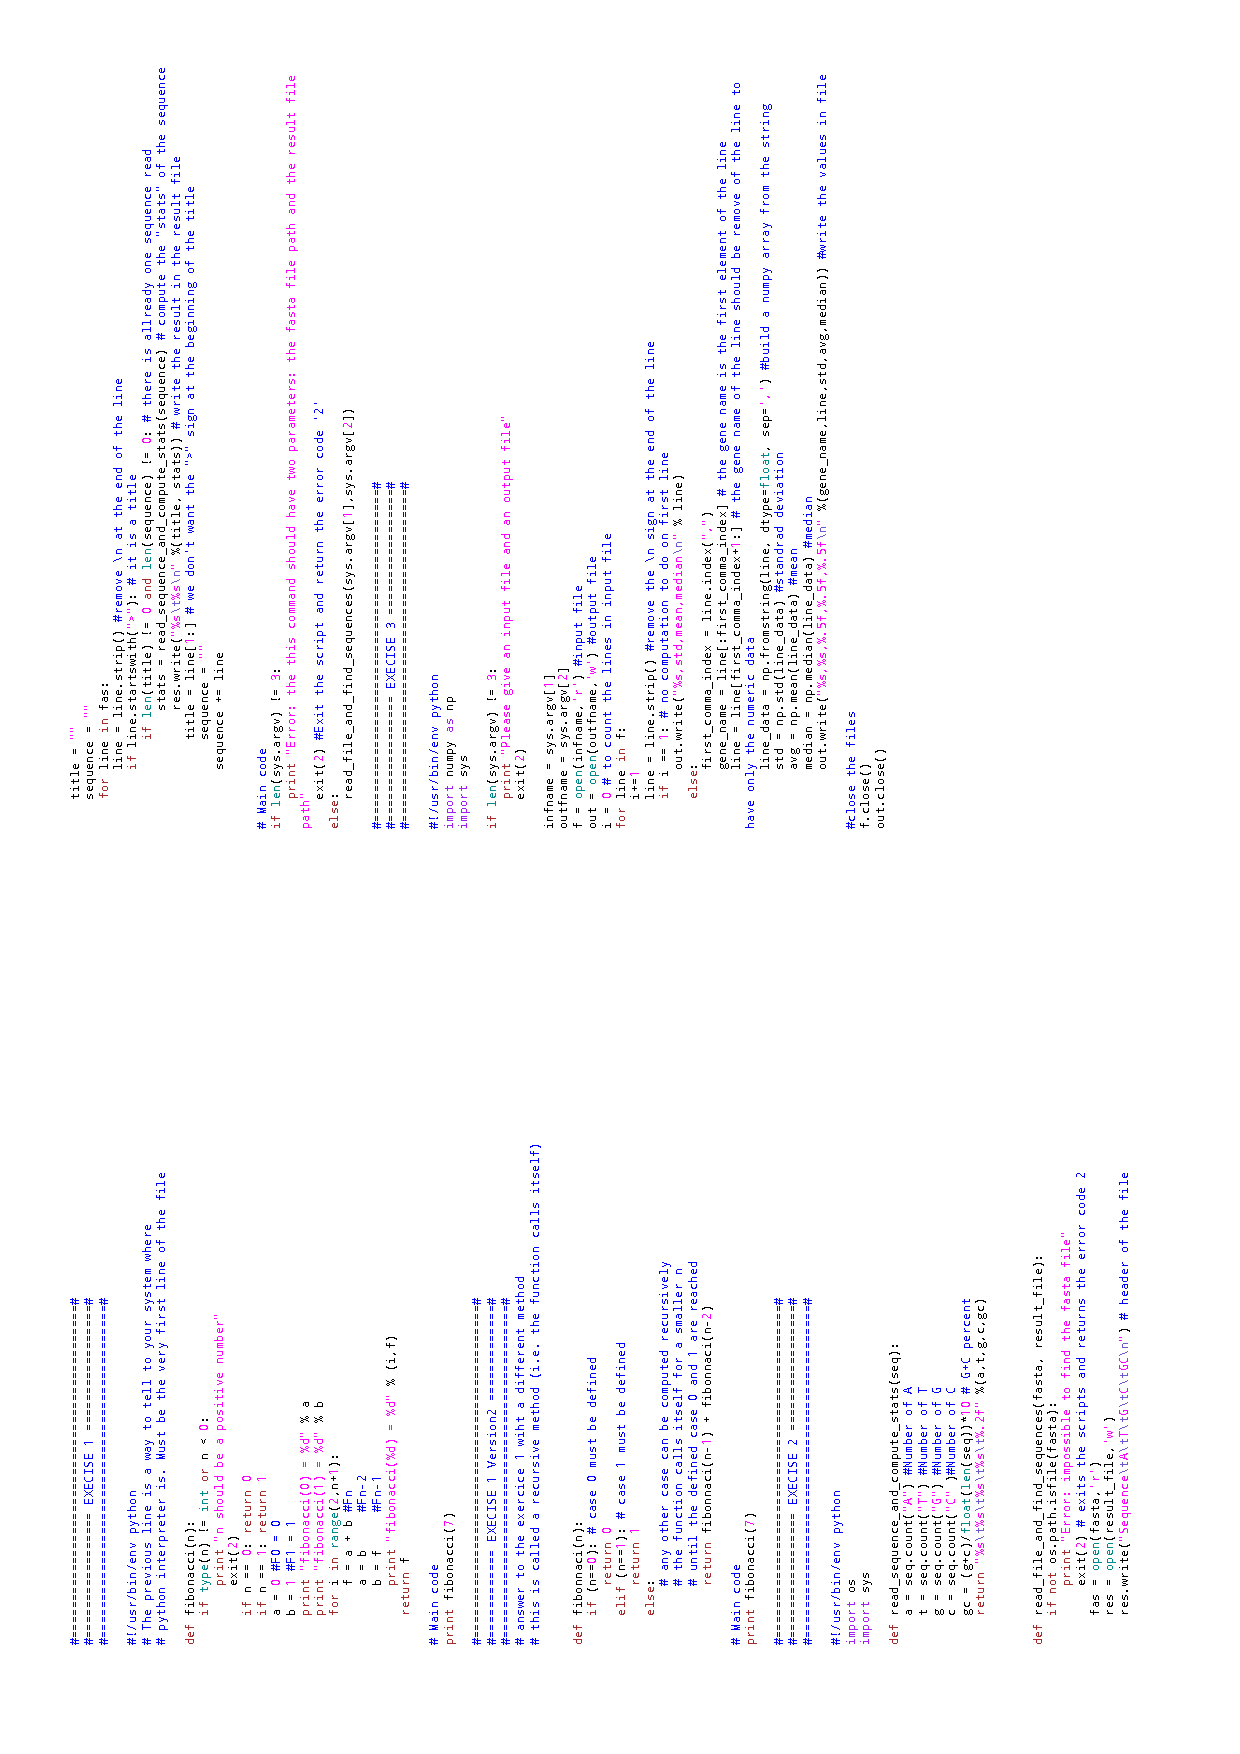
\includepdf[fitpaper=true, pages=-, offset=3cm -3.5cm ]{solutions}
\end{document}
